% Réplica local del paper «A Fast Wait-Free Solution to Read-Reclaim Races in Reference Counting» (Euro-Par 2024).
% Cuerpo: la réplica en la PC (i5-10400). Anexo: la exposición del paper (exposicion_25min.pdf, compílala antes).
% Compilar: latexmk -pdf -interaction=nonstopmode -halt-on-error replica.tex
\documentclass[aspectratio=169,11pt]{beamer}
\usepackage[spanish,es-noshorthands,es-nodecimaldot,es-tabla]{babel}
\usepackage[T1]{fontenc}
\usepackage[sfdefault,lining]{FiraSans}
\usepackage[scale=0.86]{FiraMono}
\usepackage{booktabs,tabularx,array,graphicx,pifont,xcolor,pdfpages}
\usepackage{tikz}
\usetikzlibrary{arrows.meta,positioning,calc,babel}
\hypersetup{pdftitle={Réplica: A Fast Wait-Free Solution to Read-Reclaim Races in Reference Counting},pdfauthor={},pdfcreator={},pdfproducer={},pdfsubject={},pdfkeywords={}}

% ---------- paleta (la misma de la exposición) ----------
\definecolor{tinta}{HTML}{1B2430}
\definecolor{gris}{HTML}{5B6573}
\definecolor{acento}{HTML}{C8551F}
\definecolor{hoja}{HTML}{1F5FA8}
\definecolor{ok}{HTML}{1B7F3B}
\definecolor{mal}{HTML}{B3261E}
\definecolor{suave}{HTML}{EEF1F5}
\newcommand{\si}{\textcolor{ok}{\ding{51}}}
\newcommand{\no}{\textcolor{mal}{\ding{55}}}
\newcommand{\casi}{\textcolor{acento}{$\sim$}}
\newcommand{\us}{\,\textmu s}
\newcommand{\clave}[1]{\textcolor{acento}{\textbf{#1}}}
\newcommand{\fuente}[1]{\par\vspace{2pt}{\scriptsize\color{gris}#1}}

\setbeamertemplate{navigation symbols}{}
\setbeamercolor{normal text}{fg=tinta}
\setbeamercolor{structure}{fg=hoja}
\setbeamercolor{frametitle}{fg=tinta}
\setbeamerfont{frametitle}{size=\Large,series=\bfseries}
\setbeamertemplate{frametitle}{\vspace*{8pt}\insertframetitle\par\vspace{3pt}{\color{acento}\rule{1.6cm}{2.2pt}}\vspace*{-4pt}}
\setbeamertemplate{itemize item}{\textcolor{acento}{\small$\blacktriangleright$}}
\setbeamertemplate{itemize subitem}{\textcolor{gris}{--}}
\setbeamertemplate{enumerate item}{\textcolor{acento}{\bfseries\insertenumlabel.}}
\setbeamertemplate{footline}{\leavevmode\hbox to\paperwidth{\hspace{10pt}\color{gris}\scriptsize%
  Réplica local · de Wolff, Anderson, Keller y Seletskiy · Euro-Par 2024\hfill\insertframenumber\,/\,\inserttotalframenumber\hspace{10pt}}\vspace{6pt}}
\setlength{\tabcolsep}{5pt}

\begin{document}

% =====================================================================
{\setbeamertemplate{footline}{}
\begin{frame}[plain]
  \vspace*{6mm}
  {\color{acento}\small\bfseries RÉPLICA DE PAPER EN UNA PC LOCAL}\par\smallskip
  {\fontsize{24}{28}\selectfont\bfseries A Fast Wait-Free Solution to\\ Read-Reclaim Races in Reference Counting\par}
  \medskip
  {\large\color{gris}¿Se sostienen sus afirmaciones en un Intel i5-10400 de 12 hilos?\par}
  \vfill
  {\small de Wolff, Anderson, Keller y Seletskiy · Euro-Par 2024, LNCS 14803, págs. 103--118\par}
  \smallskip
  {\small David Tamo Turpo · Jheremy Manuel Alvarez Astete · Diego Quispe Candelario\par}
  \smallskip
  {\scriptsize\color{gris}Código y resultados: github.com/davichiacustico-ux/replica-wait-free-refcount\par}
\end{frame}}

% =====================================================================
\begin{frame}{Qué afirma el paper y qué comprobamos aquí}
  \small
  \begin{tabularx}{\linewidth}{@{}>{\raggedright\arraybackslash}X >{\raggedright\arraybackslash}X c@{}}
    \toprule
    \textbf{Afirmación del paper} & \textbf{Cómo la pusimos a prueba en la PC} & \textbf{¿Se sostiene?}\\
    \midrule
    Sin carreras \emph{read-reclaim}: nunca se lee memoria liberada & AddressSanitizer y ThreadSanitizer con 8--16 hilos; versión ingenua como control & \si\\
    \emph{Wait-free}: cada recarga del peso hace $\le P$ intentos de CAS & Boceto instrumentado ($P=8$) y dos variantes rotas a propósito & \si\\
    Más rápido que los que no gastan memoria extra (fig.~5) & Pila concurrente, 6 paneles, 1--18 hilos; rivales Libstdc++, Williams y un mutex & \si\\
    \texttt{load} con la menor latencia (fig.~6) & 100\,000 muestras, $p = 1$ y $p = 12$ & \casi\\
    \bottomrule
  \end{tabularx}
  \fuente{\si{} se reproduce · \casi{} se reproduce frente a los rivales del paper, pero un mutex simple tiene mejor mediana (no mejor cola).}
\end{frame}

% =====================================================================
\begin{frame}{El problema en una diapositiva: la carrera \emph{read-reclaim}}
  \begin{columns}[c]
    \column{0.52\textwidth}
    \begin{tikzpicture}[font=\small,>=Stealth, caja/.style={draw,rounded corners=2pt,minimum width=2.2cm,minimum height=7mm}]
      \node[caja,fill=suave] (v) at (0,0) {variable \texttt{x}};
      \node[caja,fill=suave] (o) at (3.4,0) {objeto · cuenta 1};
      \draw[->,thick] (v) -- (o);
      \node[text=hoja,align=center] at (0,-1.4) {\textbf{Lector}\\1. lee la dirección};
      \node[text=mal,align=center] at (3.4,-1.4) {\textbf{Escritor}\\2. cambia \texttt{x}, cuenta $\to$ 0\\3. \textbf{libera} el objeto};
      \node[text=hoja,align=center] at (1.7,-2.75) {4. lector: cuenta$+{+}$ \ldots\ \textcolor{mal}{\bfseries sobre memoria liberada}};
    \end{tikzpicture}
    \column{0.46\textwidth}
    \begin{itemize}\small
      \item Leer el puntero y subir la cuenta son \textbf{dos pasos}; entre ambos, otro hilo puede liberar.
      \item Soluciones previas: candados (Libstdc++), \emph{lock-free} (Williams, Folly) o memoria extra (Anderson).
      \item El paper: \clave{wait-free}, sin memoria extra y rápido.
    \end{itemize}
  \end{columns}
\end{frame}

% =====================================================================
\begin{frame}{La idea en una diapositiva: el peso (talonario de tickets)}
  \begin{columns}[c]
    \column{0.5\textwidth}
    \begin{itemize}\small
      \item La variable guarda \textbf{puntero + peso} en una sola palabra de 64 bits (48 bits de dirección, el resto para el peso).
      \item El objeto ya cuenta con \clave{$C$} referencias por adelantado: el peso es lo que queda del talonario.
      \item \texttt{load} = un solo \texttt{fetch\_add} que \textbf{arranca un ticket}: leer y reservar ocurren a la vez. La carrera desaparece.
      \item Si quedan menos de $P$ tickets, se recarga con CAS; \clave{como mucho $P$ intentos} $\Rightarrow$ \emph{wait-free}.
      \item Condición R-1: $C \ge 2P$. En el paper, $C = 2^{19}$, $P = 2^{16}$.
    \end{itemize}
    \column{0.48\textwidth}\centering
    \begin{tikzpicture}[font=\small]
      \draw[fill=suave] (0,0) rectangle (6,0.8);
      \draw[fill=acento!25] (0,0) rectangle (1.6,0.8);
      \node at (0.8,0.4) {peso};
      \node at (3.8,0.4) {puntero (48 bits)};
      \node[gris,font=\scriptsize] at (0.8,-0.3) {16 (+3) bits};
      \node[gris,font=\scriptsize] at (3,1.15) {una palabra de 64 bits: un \texttt{fetch\_add} la cambia entera};
    \end{tikzpicture}
  \end{columns}
\end{frame}

% =====================================================================
\begin{frame}{La máquina: 12 hilos frente a 144}
  \small
  \begin{tabularx}{\linewidth}{@{}l X X X@{}}
    \toprule
    & \textbf{Réplica (nuestra PC)} & \textbf{Paper: rendimiento} & \textbf{Paper: latencia}\\
    \midrule
    CPU & Intel Core i5-10400, 1 socket & 4 × Xeon E7-8867 (NUMA) & Xeon w7-3465X\\
    Núcleos / hilos & 6 / \textbf{12} & 72 / 144 & 28 / 56\\
    Memoria & 24 GB (11 GB en WSL2) & 1 TB DDR4 & 128 GB DDR5\\
    Hilos probados & 1, 2, 4, 8, 12 y \textbf{18} (×1,5) & 1--216 (×1,5) & $p=1$ y $p=56$\\
    Sistema & WSL2 Ubuntu 24.04, g++ 13.3 & -- & --\\
    \bottomrule
  \end{tabularx}
  \bigskip
  \begin{itemize}\small
    \item La CPU cumple lo que el algoritmo necesita: x86-64 con \textbf{48 bits de dirección virtual} (sin LA57) y CAS de 128 bits (\texttt{cx16}, lo usa Williams).
    \item Con 12 hilos vemos el comienzo de las curvas del paper: comparamos \clave{tendencias y proporciones}, no cifras absolutas.
  \end{itemize}
\end{frame}

% =====================================================================
\begin{frame}[fragile]{Qué se ejecuta: un solo script}
  \begin{columns}[T]
    \column{0.5\textwidth}
    \small
    \begin{itemize}
      \item \textbf{Código de los autores}, sin tocar: submódulo \texttt{codigo/autores} (commit \texttt{8540c58}).
      \item \textbf{Rivales}: \texttt{std::atomic<shared\_ptr>} de GCC (Libstdc++, con candado), \textbf{Williams} (\emph{split refcount}, \emph{lock-free}, submódulo) y un \texttt{std::mutex}.
      \item \textbf{Pruebas propias}: \texttt{estres\_asan.cpp}, boceto con variantes rotas, \texttt{bench.cpp} (pila concurrente y latencia).
    \end{itemize}
    \column{0.48\textwidth}
\begin{semiverbatim}\scriptsize
cd exposicion_paper/codigo
bash ejecutar_pruebas.sh   # ~4 min
\end{semiverbatim}
    \small Compila con g++ y guarda en \texttt{capturas/}:
    \begin{enumerate}\small
      \item entorno y demo de los autores
      \item ASan y TSan (ingenua / autores)
      \item boceto y variantes rotas
      \item rendimiento (CSV) y latencia (CSV)
    \end{enumerate}
  \end{columns}
\end{frame}

% =====================================================================
\begin{frame}{Corrección (1): la carrera existe y el algoritmo la evita}
  \centering
  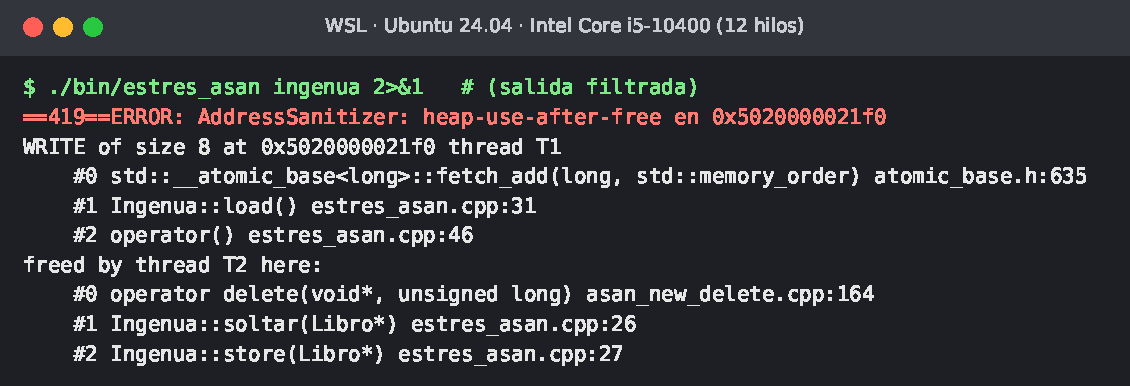
\includegraphics[width=0.92\linewidth,height=0.48\textheight,keepaspectratio]{graficos/captura_asan_ingenua.pdf}\par\smallskip
  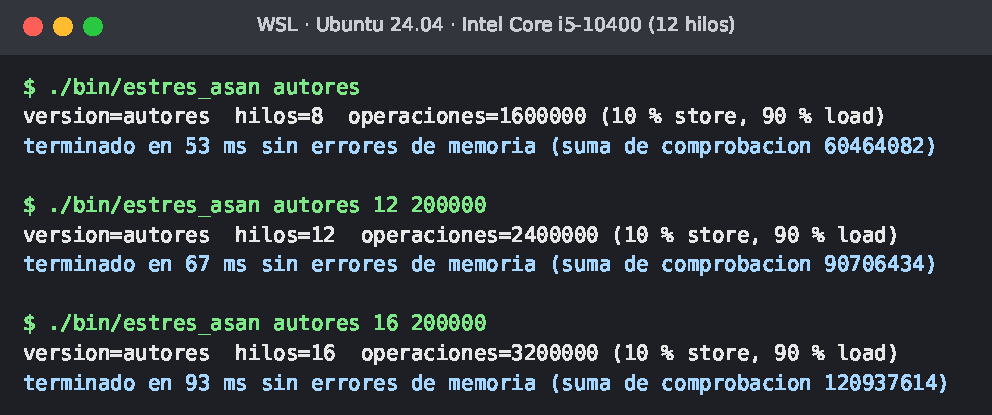
\includegraphics[width=0.66\linewidth,height=0.17\textheight,keepaspectratio]{graficos/captura_asan_autores.pdf}
  \fuente{Arriba, versión ingenua: \emph{heap-use-after-free} en \texttt{load()} (\texttt{fetch\_add}) sobre memoria liberada por otro hilo en \texttt{store()}. Abajo, código de los autores: 1,6 M operaciones (8 hilos), 2,4 M (12) y 3,2 M (16), \textbf{0 errores}.}
\end{frame}

% =====================================================================
\begin{frame}{Corrección (2): la cota \emph{wait-free} y por qué cada pieza importa}
  \small
  \begin{tabularx}{\linewidth}{@{}l X r r r@{}}
    \toprule
    \textbf{Versión} ($P = 8$, 8 hilos, 4 M ops.) & \textbf{Qué cambia} & \textbf{Errores} & \textbf{Máx. CAS} & \\
    \midrule
    Paper & $C = 2P = 16$, con salida temprana & 0 & 8 $\le P$ & \si\\
    Sin salida temprana & la recarga no se rinde al ver que otro ya recargó & 0 & \textbf{55} $> P$ & \no\\
    $C = P$ & incumple R-1 ($C \ge 2P$) & \textbf{63\,101} & 8 & \no\\
    Ingenua & leer y subir la cuenta en dos pasos & \textbf{632\,125} & -- & \no\\
    \bottomrule
  \end{tabularx}
  \bigskip
  \begin{itemize}\small
    \item La salida temprana es lo que hace la recarga \emph{wait-free}; R-1 es lo que la hace correcta.
    \item ThreadSanitizer: código de los autores sin avisos con 8 hilos.
    \item Es una comprobación empírica (no una demostración: la prueba está en el §4.1 del paper) y sobre el boceto, no sobre el código de los autores.
  \end{itemize}
\end{frame}

% =====================================================================
\begin{frame}{Rendimiento: pila concurrente (como la fig.~5)}
  \centering
  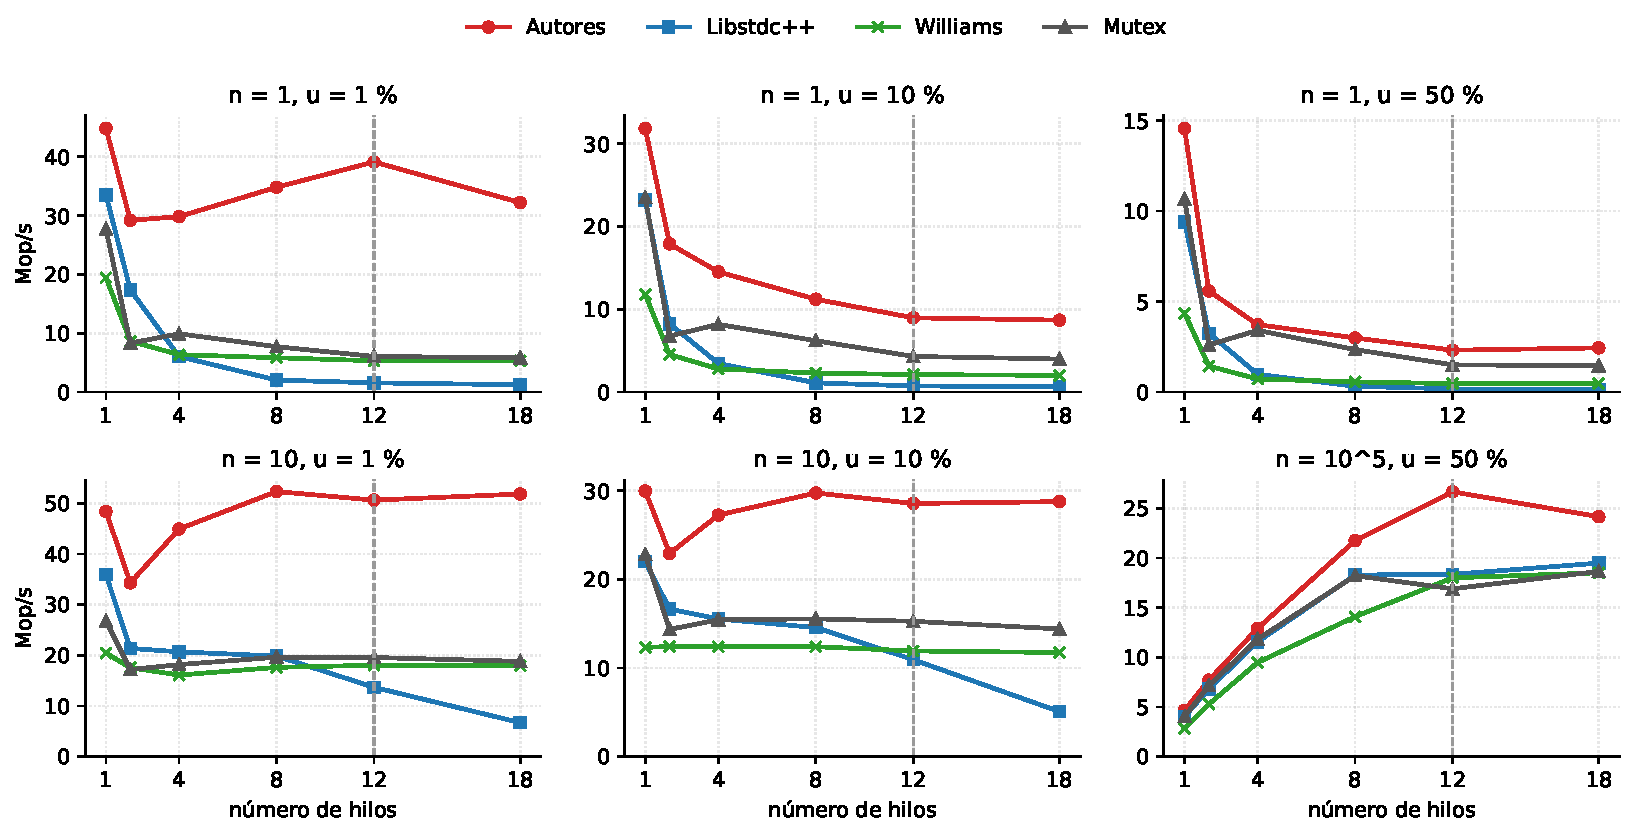
\includegraphics[width=0.98\linewidth,height=0.64\textheight,keepaspectratio]{graficos/local_rendimiento.pdf}
  \fuente{$n$ pilas, $u$\,\% de actualizaciones, 1 s por punto. La línea discontinua marca 12 hilos (hilos por hardware); 18 = sobresuscripción ×1,5, como 216 = 1,5 × 144 en el paper.}
\end{frame}

% =====================================================================
\begin{frame}{Rendimiento: las cifras a 12 hilos (Mop/s)}
  \small
  \begin{tabularx}{\linewidth}{@{}l r r r r X@{}}
    \toprule
    \textbf{Panel} & \textbf{Autores} & \textbf{Williams} & \textbf{Libstdc++} & \textbf{Mutex} & \textbf{Lectura}\\
    \midrule
    $n=1,\ u=1$ & \textbf{39,1} & 5,3 & 1,6 & 6,1 & una sola pila: máxima contención\\
    $n=1,\ u=50$ & \textbf{2,3} & 0,5 & 0,2 & 1,5 & la mitad son CAS: todos caen\\
    $n=10,\ u=1$ & \textbf{50,6} & 18,0 & 13,7 & 19,6 & poca contención\\
    $n=10^5,\ u=50$ & \textbf{26,7} & 18,0 & 18,4 & 16,9 & casi sin contención\\
    \bottomrule
  \end{tabularx}
  \bigskip
  \begin{itemize}\small
    \item \textbf{Autores gana en los 6 paneles} a todos los rivales sin memoria extra.
    \item Frente a Williams, el antecesor directo: \clave{$\approx$7×} con una pila a 12 hilos; el paper reporta $\approx$7× con 144 hilos.
    \item Con 1 hilo nuestra PC da más Mop/s que el servidor del paper (44,8 frente a $\approx$9): un solo socket sin NUMA y relojes más altos. Por eso no comparamos valores absolutos.
  \end{itemize}
\end{frame}

% =====================================================================
\begin{frame}{Latencia: un hilo mide, los demás escriben (como la fig.~6)}
  \centering
  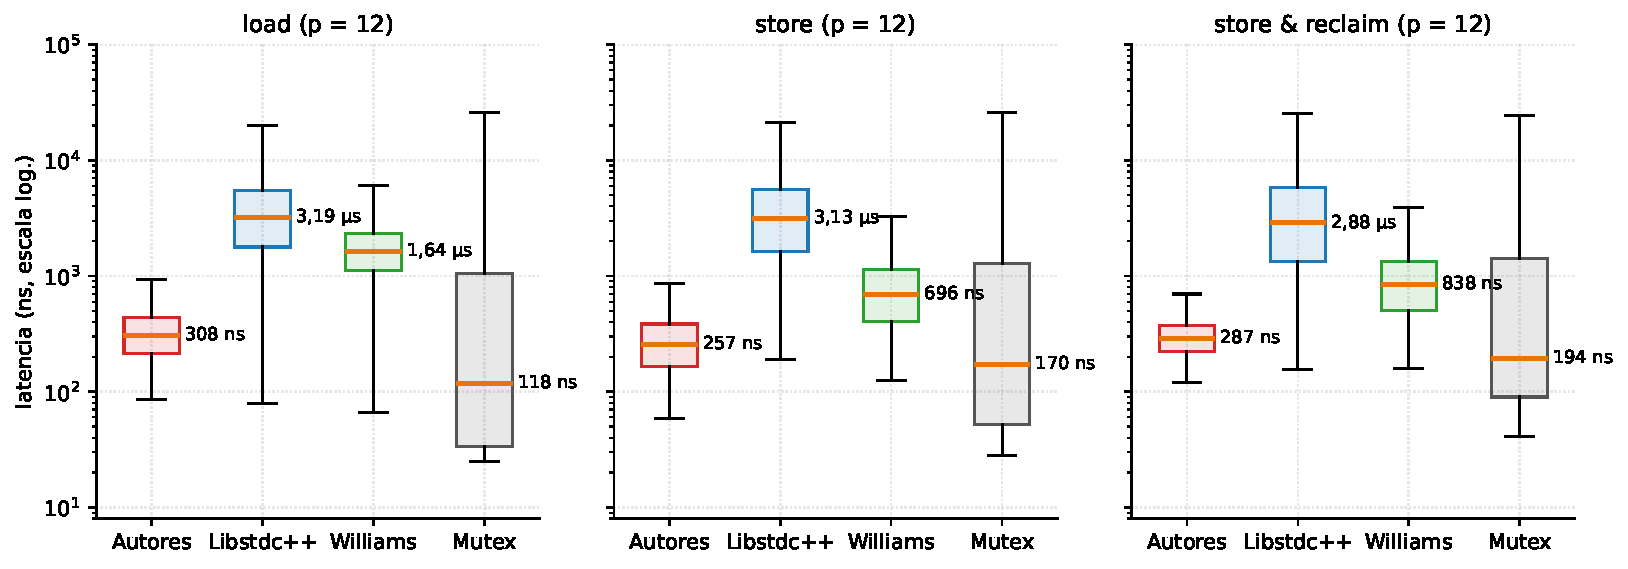
\includegraphics[width=0.98\linewidth,height=0.66\textheight,keepaspectratio]{graficos/local_latencia.pdf}
  \fuente{$p = 12$: 1 hilo mide y 11 hacen \texttt{store} sin parar. Caja: percentiles 25--75; bigotes: 1 y 99. Escala logarítmica.}
\end{frame}

% =====================================================================
\begin{frame}{Latencia de \texttt{load}: mediana y cola}
  \small
  \begin{tabularx}{\linewidth}{@{}l r r r X@{}}
    \toprule
    \textbf{Implementación} & \textbf{$p=1$} & \textbf{$p=12$ mediana} & \textbf{$p=12$ p99} & \\
    \midrule
    Autores & \textbf{6,3 ns} & 308 ns & \textbf{0,93\us} & \emph{wait-free}: un \texttt{fetch\_add}\\
    Williams & 31,7 ns & 1,64\us & 6,1\us & \emph{lock-free}: reintenta\\
    Libstdc++ & 13,6 ns & 3,19\us & 20\us & candado interno\\
    Mutex & 6,4 ns & \textbf{118 ns} & \textcolor{mal}{25,8\us} & a veces entra sin esperar, a veces espera mucho\\
    \bottomrule
  \end{tabularx}
  \bigskip
  \begin{itemize}\small
    \item Frente a los rivales del paper, Autores tiene la menor latencia, con y sin contención (paper, $p=1$: 23 ns frente a 29 ns de Libstdc++).
    \item El mutex gana en \emph{mediana} pero su \clave{cola es 28 veces peor}: eso es justo lo que \emph{wait-free} promete evitar.
    \item Ojo: con el mutex, p1 y p25 salen a 0 ns tras descontar el coste del reloj (47 ns): está por debajo de lo que medimos bien.
  \end{itemize}
\end{frame}

% =====================================================================
\begin{frame}{Paper frente a réplica}
  \small
  \begin{tabularx}{\linewidth}{@{}>{\raggedright\arraybackslash}X >{\raggedright\arraybackslash}X >{\raggedright\arraybackslash}X c@{}}
    \toprule
    \textbf{Aspecto} & \textbf{Paper} & \textbf{Réplica} & \\
    \midrule
    Corrección & demostración (§4.1) & ASan/TSan sin errores; la ingenua falla & \si\\
    Cota de CAS & $\le P$ (teorema) & 8 $\le P$; sin salida temprana, 55 & \si\\
    Frente a Williams & $\approx$7× más rápido (1 pila) & $\approx$7× más rápido (1 pila) & \si\\
    Frente a Libstdc++ & mucho más rápido & 24× (1 pila, 12 hilos) & \si\\
    \texttt{load} con contención & la menor de todas & la menor salvo la mediana del mutex & \casi\\
    Frente a Anderson / Folly & Anderson gana con mucha contención & no medido & --\\
    \bottomrule
  \end{tabularx}
\end{frame}

% =====================================================================
\begin{frame}{Diferencias que declaramos}
  \begin{itemize}\small
    \item \textbf{Escala}: 12 hilos y 1 socket frente a 144 hilos y 4 sockets NUMA. No evaluamos la coherencia entre sockets.
    \item \textbf{Rivales}: añadimos Williams; Folly y Anderson quedan como trabajo futuro. Anderson es el único que el paper ve ganar (con mucha contención).
    \item \textbf{Paneles}: el último usa $n = 10^5$ pilas; el paper usa $10^6$.
    \item \textbf{Repeticiones}: una pasada por punto (el plan pide 3 y la mediana).
    \item \textbf{Mutex}: no está en el paper; lo usamos como referencia sencilla.
    \item \textbf{TSan}: con 16 hilos falla al arrancar (\emph{unexpected memory mapping}, un problema conocido de TSan con la aleatorización de direcciones del kernel, no del algoritmo).
  \end{itemize}
\end{frame}

% =====================================================================
\begin{frame}{Conclusión}
  \begin{itemize}
    \item En una PC normal se reproduce lo esencial del paper: \clave{ninguna lectura de memoria liberada}, \clave{cota de $P$ intentos} y \clave{el más rápido sin memoria extra}.
    \item Cada pieza del algoritmo es necesaria: quitar la salida temprana rompe la cota; $C = P$ rompe la memoria.
    \item La ventaja frente al \emph{split refcount} (Williams) es la misma proporción que en el paper, con 12 veces menos hilos.
    \item Lo que no podemos decir: cómo escala en 144 hilos con NUMA ni cómo queda frente a Anderson.
  \end{itemize}
  \vfill
  \centering{\small\color{gris}Todo se puede ejecutar en vivo: \texttt{EN\_VIVO.md} y las tareas de VS Code.}
\end{frame}

% =====================================================================
{\setbeamertemplate{footline}{}
\begin{frame}[plain]
  \vfill{\color{acento}\large\bfseries Anexo}\par\medskip
  {\fontsize{30}{34}\selectfont\bfseries El paper explicado}\par\bigskip
  {\color{gris}La exposición completa del paper: el problema, el algoritmo, la demostración y los experimentos originales.}\vfill
\end{frame}}

\includepdf[pages=2-]{exposicion_25min.pdf}

\end{document}
